\documentclass{article}

\usepackage[final, nonatbib]{neurips_2024}
\usepackage[numbers,compress]{natbib}
\usepackage[T1]{fontenc}
\usepackage[utf8]{inputenc}
\usepackage{amsmath,amssymb}
\usepackage{graphicx}
\usepackage{booktabs}
\usepackage{microtype}
\usepackage{hyperref}
\hypersetup{hidelinks}

\title{Topology Is Lossy: Skeletonization Discards Discriminative\\
       Stroke Information for CNN Digit Recognition}

\author{%
  Attila Torda \\
  Independent Researcher \\
}

\begin{document}
\maketitle

\begin{abstract}
Skeletonization---reducing a stroke to its one-pixel medial axis---is an appealing
pre-processing step for handwritten digits: it is stroke-thickness invariant, compact, and
classical. We test, in a controlled study, whether it actually helps a convolutional digit
classifier, and find a clean negative. Across four standard thinning algorithms (Zhang--Suen,
Guo--Hall, Lee, medial-axis), a CNN trained on skeletonized MNIST trails the same CNN on raw
pixels by $0.9$--$1.2$ percentage points (best skeleton $98.11\%$ vs raw $99.03\%$; $3$ seeds).
The loss is not recoverable: adding the skeleton as a second input channel alongside the raw
image (\emph{fusion}) does \emph{not} beat raw pixels alone ($98.98\%$ vs $99.03\%$), and adding
Hough line features to the skeleton changes accuracy by $+0.01$~pp. The degradation concentrates
on stroke-width- and density-sensitive digits (3, 5, 9, 8), and the most expensive skeletonizer
(medial-axis, $100\times$ slower) is no more accurate. The takeaway is simple and, we argue,
useful to state plainly: for digit recognition, stroke width and grayscale intensity carry
discriminative information that thinning throws away, and a topological representation alone is
strictly worse---a result that should temper the recurring intuition that skeletons are a good
front-end for digit CNNs.
\end{abstract}

\section{Introduction}
Thinning a binary shape to its medial axis \cite{Blum1967} is a classical operation with an
intuitive appeal for handwriting: it normalises stroke thickness, yields a compact graph-like
representation, and has fast parallel algorithms \cite{ZhangSuen1984,GuoHall1989}. It is
therefore a recurring idea to feed \emph{skeletonized} digits to a neural classifier. We ask the
direct empirical question---does it help?---and report a controlled negative: on MNIST
\cite{LeCun1998}, skeletonization consistently \emph{hurts} a CNN, the loss is not recovered by
fusing the skeleton with the raw image, and it traces to information (stroke width, intensity)
that thinning is designed to remove. Negative results like this are worth recording: the
intuition that ``topology is enough'' for digits is common, and a clean controlled refutation
saves re-implementation effort.

\section{Setup}
We use one backbone (a small two-block CNN, \texttt{SimpleCNN}) and vary only the input.
\textbf{Inputs:} raw $28\times28$ grayscale; skeletons from four algorithms---Zhang--Suen
\cite{ZhangSuen1984}, Guo--Hall \cite{GuoHall1989}, Lee \cite{Lee1994}, and a medial-axis
transform---each binarised at a fixed threshold; optional Hough-line channels
\cite{DudaHart1972}; and a two-channel \emph{fusion} of raw $+$ Guo--Hall skeleton. All
configurations share epochs, batch size, learning rate, and architecture; we report mean
$\pm$ std test accuracy over $3$ seeds.

\section{Results}
\paragraph{Every skeletonizer underperforms raw pixels (Table~\ref{tab:overall},
Fig.~\ref{fig:skel}).}
The best skeleton (Guo--Hall, $98.11\%$) trails raw pixels ($99.03\%$) by $0.92$~pp; the worst
(Zhang--Suen, $97.81\%$) by $1.22$~pp. The gap exceeds the seed-to-seed std ($\leq 0.11$) by an
order of magnitude, so it is not noise.

\paragraph{The loss is not recoverable.}
Two controls rule out ``the skeleton adds complementary information the CNN just needs help
using.'' (i)~\textbf{Fusion}: giving the network \emph{both} the raw image and its skeleton as
two channels yields $98.98\%$---statistically indistinguishable from, and numerically below, raw
alone ($99.03\%$). The skeleton channel contributes nothing the pixels do not already carry.
(ii)~\textbf{Hough lines}: appending Hough line-segment features to the skeleton moves accuracy by
$+0.01$~pp across all four thinners---within noise.

\begin{table}[t]
\caption{MNIST test accuracy (\%, mean $\pm$ std over $3$ seeds) and skeletonization cost.
Every topological input trails raw pixels; fusion does not recover the gap.}
\label{tab:overall}
\centering
\begin{tabular}{@{}lccr@{}}
\toprule
Input & Channel & Accuracy & Skel.\ time (s) \\
\midrule
Raw pixels                 & raw            & $\mathbf{99.03 \pm 0.06}$ & --- \\
\midrule
Guo--Hall \cite{GuoHall1989}      & skeleton       & $98.11 \pm 0.09$ & 26 \\
\;\; + Hough \cite{DudaHart1972}  & skeleton+hough & $98.12 \pm 0.09$ & 26 \\
Lee \cite{Lee1994}                & skeleton       & $98.02 \pm 0.07$ & 8 \\
medial-axis                       & skeleton       & $97.95 \pm 0.11$ & 2978 \\
Zhang--Suen \cite{ZhangSuen1984}  & skeleton       & $97.81 \pm 0.04$ & --- \\
\midrule
Raw $+$ Guo--Hall (fusion) & raw+skeleton   & $98.98 \pm 0.05$ & 26 \\
\bottomrule
\end{tabular}
\end{table}

\paragraph{Where the information goes (Table~\ref{tab:perclass}, Fig.~\ref{fig:skel} right).}
The degradation is not uniform: digits $0$ and $1$ are essentially unaffected, while $3$
($-1.7$~pp), $5$ ($-1.6$), $9$ ($-1.2$), $4$ ($-1.2$) and $8$ lose the most under Guo--Hall;
under Zhang--Suen, digit $8$ collapses by $3.1$~pp ($98.8\to95.7$). These are exactly the digits
whose identity depends on stroke \emph{thickness}, loop \emph{density}, and intersection detail
(open vs.\ closed loops, doubled strokes)---precisely what one-pixel thinning erases. Fusion's
per-class accuracy tracks raw, confirming the skeleton channel adds nothing.

\begin{table}[t]
\caption{Per-class accuracy (\%, mean over $3$ seeds): raw vs.\ Guo--Hall skeleton vs.\ fusion.}
\label{tab:perclass}
\centering
\small
\begin{tabular}{@{}lcccccccccc@{}}
\toprule
 & 0 & 1 & 2 & 3 & 4 & 5 & 6 & 7 & 8 & 9 \\
\midrule
raw       & 99.7 & 99.5 & 98.9 & 99.3 & 99.1 & 99.0 & 98.7 & 99.3 & 98.8 & 97.9 \\
skeleton  & 99.8 & 99.2 & 98.5 & 97.6 & 97.9 & 97.4 & 98.0 & 98.2 & 97.6 & 96.7 \\
fusion    & 99.7 & 99.8 & 99.0 & 99.2 & 99.3 & 98.9 & 98.3 & 99.2 & 98.3 & 98.1 \\
\bottomrule
\end{tabular}
\end{table}

\paragraph{Cost.} The medial-axis transform is $\sim\!100\times$ slower than Guo--Hall
($2978$\,s vs.\ $26$\,s to skeletonize the dataset) and \emph{less} accurate---there is no
accuracy/cost frontier on which any skeletonizer dominates raw pixels.

\begin{figure}[t]
\centering
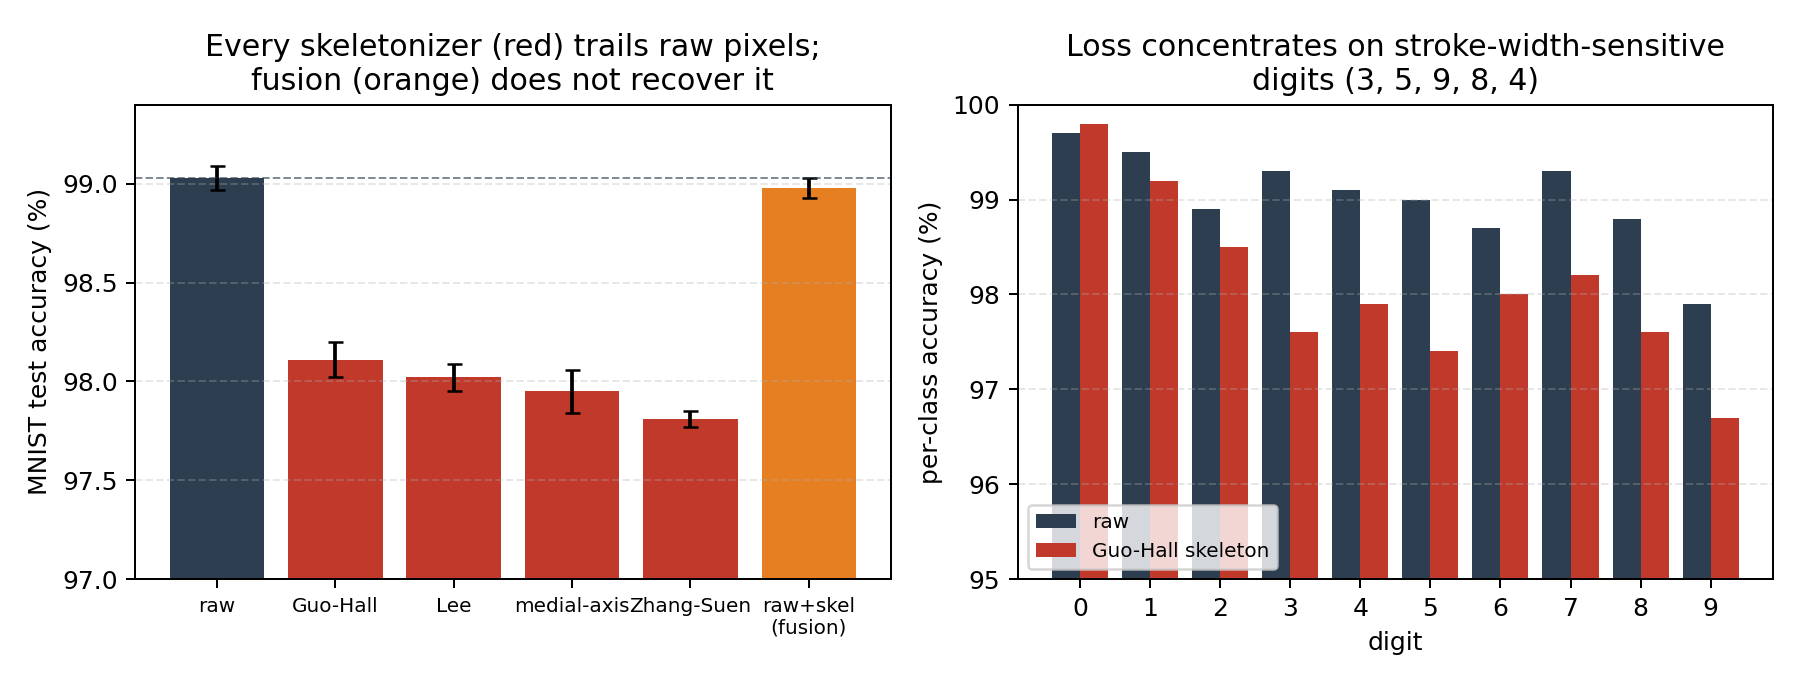
\includegraphics[width=0.95\linewidth]{figures/fig_skeleton_negative.png}
\caption{Left: every thinning algorithm (red) trails raw pixels (dashed line); the raw$+$skeleton
fusion (orange) does not recover the gap. Right: per-class accuracy, raw vs.\ Guo--Hall skeleton;
the loss concentrates on stroke-width/density-sensitive digits.}
\label{fig:skel}
\end{figure}

\section{Discussion}
The result is unsurprising in hindsight but worth stating because the opposite intuition is
common. Skeletonization is \emph{designed} to be invariant to stroke width; for digit
\emph{recognition}, stroke width and grayscale intensity are not nuisances but \emph{features}
(they separate a thick-looped $8$ from a $0$, a heavy $5$ from a $6$, etc.). Discarding them is a
strict information loss that a CNN---which already learns its own thickness-tolerant features
from raw pixels \cite{Simard2003}---cannot recover, and that re-supplying the skeleton as a side
channel does not help. We emphasise the \emph{controlled} nature of the claim: same backbone,
same training, four thinners, a fusion control, and a Hough control all point the same way.

\paragraph{Scope.} This is a statement about \emph{supervised, data-rich} digit recognition with
a CNN. It does \emph{not} say skeletons are useless in general: thickness-invariant topological
descriptors can be competitive in the extreme low-data / one-shot regime and can add robustness
under stroke-width corruption, where the CNN's pixel features are unreliable. The negative is
specifically that, when you have pixels and labels, thinning them first only throws information
away.

\section{Conclusion}
For supervised CNN digit recognition, skeletonization is a lossy front-end: across four thinning
algorithms it costs $\sim\!1$~pp versus raw pixels, the loss concentrates on stroke-width-sensitive
digits, and it is recovered neither by raw$+$skeleton fusion nor by Hough line features. Topology
alone is not enough; keep the pixels.

\begin{ack}
Reproducibility: \texttt{scripts/run\_skeleton\_experiment.py} (all configurations, $3$ seeds);
raw numbers in \texttt{experiments/reports/skeleton\_comparison.md}; skeletonizers in
\texttt{src/skeleton/}.
\end{ack}

\bibliographystyle{plainnat}
\bibliography{skeleton_refs}

\end{document}
